% Written by Martin Pasquier (Marty42780)

Le site web est une tache secondaire du projet, mais il est tout de même important pour la communication et la promotion du jeu.
Il est essentiel pour permettre aux joueurs de découvrir le jeu, de suivre son développement et de le télécharger.
C'est l'outils central de la partie communication du projet, et il est donc important de le maintenir à jour dse dernières informations sur le jeu.
\\

\subsubsection*{\hspace*{0.6cm}Avancement du site web}


Sa phase de développement est finie, il est maintenant en attente de contenu du jeu et d'être publié.
En effet du contenu du jeu tel que des images ou des vidéos de gameplay sont nécessaires pour le site web, et ces éléments ne sont pas encore prêts. En attente de ces éléments, le site web utilise des images et des vidéos de démonstration appelés "\textit{placeholders}".


\begin{figure}[H]
    \centering
    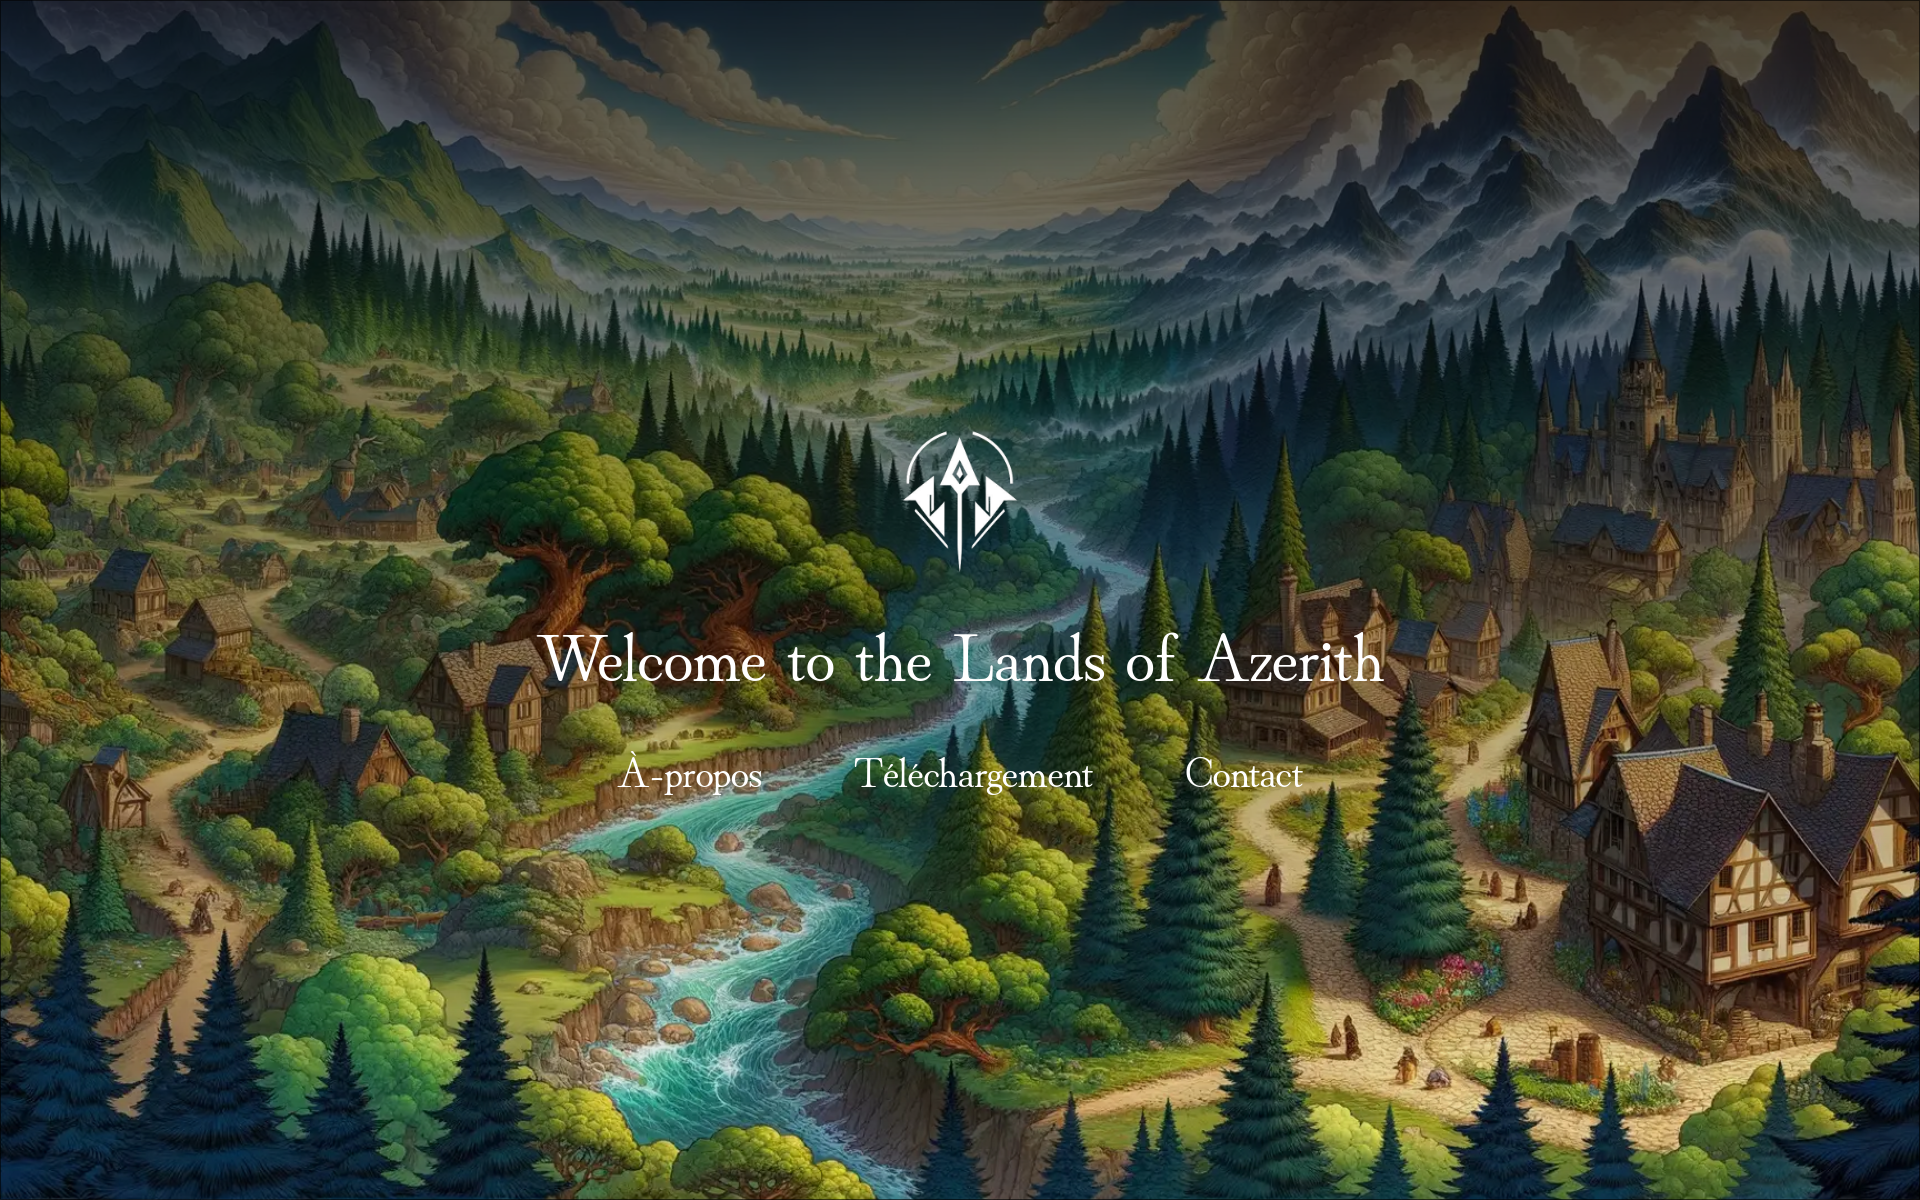
\includegraphics[width=0.8\textwidth]{2.game/assets/website1.png}
    \caption{Page d'accueil du site web, elle représente bien la simplicité voulu pour le site web.}
    \label{fig:website1}
\end{figure}

Comme le montre la \ref*{fig:website1}, le site web est simple et épuré. 
Il est composé d'une seule page, laissant l'utilisateur scroller pour découvrir les différentes sections.
Elle possède un menu de navigation qui permet de se rendre directement aux sections les plus importantes du site web, et un pied de page avec des liens vers les réseaux sociaux et le dépôt de code source du jeu.
\\

Les différentes sections sont les suivantes :

- "À propos", cette partie présente le jeu, son style et le concept associé

- "Téléchargement", pour télécharger le jeu pour les différentes plateformes

- "Contact", pour contacter l'équipe de développement en redirigeant l'utilisateur vers une adresse mail ou le dépôt GitHub du projet


\subsubsection*{\hspace*{0.6cm}Technologies utilisées}

Le site possède son propre dépôt de code source sur \textit{GitHub} à l'adresse \url{https://github.com/StonksIndustries/Azerith_Website}. 

Nous avons utilisé l'éditeur de code VSCode pour développer le site web car il offre de nombreux outils très outils pour cela. On peut citer l'intégration avec \textit{GitHub}, les extensions pour le développement web, et les outils de débogage intégrés.
\\

Le site web est développé en HTML, SCSS et JS, et est compilé avec Parcel. 
Leur choix a été motivé par leur simplicité et leur popularité, qui permettent de trouver facilement de l'aide en cas de problème. 
Parcel permet de compiler le site web sans aucune configuration et une très bonne optimisation des fichiers. 
Le \textit{SCSS}, remplace le \textit{CSS} pour permettre une meilleure organisation du code et une meilleure maintenabilité. 
Le JS est utilisé pour les animations et les interactions avec le visiteur.
\\

Il sera automatiquement compilé et publié grâce aux outils \textit{GitHub Actions} et \textit{GitHub Pages}. 
L'usage de ces outils permet de simplifier la publication du site web, et de le mettre à jour automatiquement à chaque modification du code source. 
Chaque nouvelle versions envoyés par un développeur est automatiquement compilée et publiée sur le site web si aucune erreur n'est détectée.

\subsubsection*{\hspace*{0.6cm}Objectifs futurs}

Une fois les phases de développement et de publication terminées, le site web sera mis à jour régulièrement avec les dernières informations sur le jeu. Cela comprend les étapes de développement, les nouvelles fonctionnalités et les correctifs de bugs.
\\

Des améliorations sont cependant possibles, on peut lister les suivantes:

- Compatibilité avec les appareils mobiles ("\textit{responsive design}")

- Écran de chargement et animations

- Plus d'interactivité avec le visiteur (formulaire de contact, \textit{sliders} interactifs, etc.)

